\lhead{\begin{tikzpicture}[remember picture, overlay]
    \node [anchor=100,inner sep=0] (imagenIZQUIERDA) at (current page header area.north){\includegraphics[width=18cm]{img/Encabezado.PNG}};
    \end{tikzpicture}}
    \rhead{Gómez-Hernández}
    \rfoot{\begin{tikzpicture}[remember picture, overlay]
    \node [anchor=140,inner sep=0] (imagenDERECHA) at (current page footer area.south){\includegraphics[width=18cm]{img/Foot.PNG}};
    \end{tikzpicture}}
    %----------------------------------------------------------------------------------------
    \lfoot{ \thepage}
    % \renewcommand{\labelenumi}{\alph{enumi}.)} 
    %----------------------------------------------------------------------------------------
    %----------------------------------------------------------------------------------------
    %	TITLE SECTION
    %----------------------------------------------------------------------------------------
    
    \setlength{\droptitle}{-5\baselineskip} % Move the title up
    \title{\textbf{Estudio de tiempos y movimientos en el ensamble de un circuito electrónico utilizando diferentes métodos para su optimización }} % Article title
    
     \author{ 
     \textsc{Gómez-Hernández, Manuel}\\ 
    %  Afiliación:
     \texttt{ Instituto Tecnológico de Querétaro } \\ 
     \texttt{ Tecnológico Nacional de México } \\ 
     \texttt{Querétaro, México}\\ 
     \texttt{l22140897@queretaro.tecnm.mx} 
     \and 
     \textsc{Ángeles-Hurtado, Luis Alberto}\\ 
    %  Afiliación:
     \texttt{ Instituto Tecnológico de Querétaro } \\ 
     \texttt{ Tecnológico Nacional de México } \\ 
     \texttt{Querétaro, México}\\ 
     \texttt{alb3rt0.ah@gmail.com} 
    }
    
    
    %----------------------------------------------------------------------------------------
    
    % \begin{document}
    
    % Print the title
    \maketitle
    \thispagestyle{fancy}
    
    %----------------------------------------------------------------------------------------
    %	ARTICLE CONTENTS
    %----------------------------------------------------------------------------------------
    
    % \section*{Resumen}
    % \textit{Palabras clave:}
    % El resumen (ancho de página) deberá contener entre 100 y 200 palabras tipo Adobe Devangari 11 puntos.
    
    \begin{abstract}
    \noindent 
    El resumen (ancho de página) deberá contener entre 100 y 200 palabras tipo Adobe Devangari 11 puntos.
    
    \end{abstract}
    % 
    % 
    \textbf{\textit{Palabras clave}}: {Exactitud, precisión, estudio, tiempos, movimientos, optimización.}
    
    
    \section{Introducción}
    
    % Define estudio de tiempos y movimientos
    El Estudio de Tiempos y Movimientos es una técnica clave en la gestión de la eficiencia operativa, que integra dos enfoques fundamentales: el Estudio de Tiempos, desarrollado por Frederick W. Taylor, que implica la medición y análisis cronométrico de tareas específicas, y el Estudio de Movimientos, creado por Frank y Lillian Gilbreth, que se centra en la optimización cinética de los movimientos laborales \cite{Maynards}.
    % Define que es ensamble
    Haciendo presencia en la incorporación de un ensamble, integrando varias piezas y componentes individuales asegurando la implementación de un circuito electrónico. Proceso el cual se determinara, seleccionara y ajustaran su variables buscando la optimización de dicho ensamble identificando el tiempo ciclo, tiempo estándar, ejerciendo diversos métodos \cite{glossar_item24}. 
    % Define que es circuito electronico
    Un circuito electrónico es un sistema de componentes eléctricos conectados que gestionan corriente para realizar funciones específicas. Incluye elementos como resistencias, condensadores, inductores, transistores y diodos \cite{fadesaing_circuitos}.
    % Define optimización
    La optimización se entiende como el proceso de encontrar la forma más eficiente de ejecutar una actividad. En este contexto, nos enfocamos en mejorar la eficiencia del tiempo de ensamblaje \cite{significados_optimizacion}.
    % Define metodos de tiempos predeterminados
    Para llevar a cabo este proyecto, es necesario utilizar varias herramientas, como el método de tiempos predeterminados. Este método se define como un conjunto de reglas o procedimientos que permiten establecer de antemano la secuencia de eventos \cite{H.B.MAYNARD}
    % Al final se debe hacer alisión al proyecto de investigación 
    Como objetivo general, se pretende desarrollar competencias en las áreas de ingeniería de producción, diseño de productos y control de calidad.
    
%%%%%%%%%%%%%%%%%%%%%%%%Justificación%%%%%%%%%%%%%%%%%%%%%%%% 
   
    
    \section{Justificación}

% Cuantos tipos de manufactura existen?
Ciertamente, a lo largo de los siglos XIX y XX, se han visto tres grandes transformaciones industriales que han impulsado el progreso tecnológico. La fabricación, durante estas revoluciones, ha experimentado avances significativos. En el presente, observamos una variedad de enfoques en la manufactura, cada uno en continua evolución a lo largo del tiempo y aplicable en diversas ramas industriales. 
Para ser más específicos, podemos identificar al menos seis variantes de manufactura que se emplean en distintos sectores \cite{industrialrevolutions}.
% Cuantas empresas de manufactura existen en Mundo?
La cantidad exacta de empresas de manufactura en el mundo no puede determinarse con precisión debido a la diversidad y complejidad de la industria. Sin embargo, el Banco Mundial elabora una lista de países según su producción manufacturera. En 2019, el valor total de la producción manufacturera alcanzó los 13,739,251 millones de dólares estadounidenses.
% Cuantas empresas de manufactura existen en México?
En el informe de producción manufacturera del Banco Mundial, México destaca como el séptimo país con una cifra de 314,701 millones de dólares en el año 2020. Este dato refleja una tendencia ascendente en el desarrollo y crecimiento de la industria manufacturera mexicana, según lo indicado en el análisis gráfico proporcionado por la institución.
% Cuantas empresas de manufactura existen en Querétaro?
Se estima que hay al menos 7,649 empresas dedicadas a la manufactura.


%%%%%%%%%%%%%%%%Descripción del problema%%%%%%%%%%%%%%%%%%%%%%%%%%% 
    
    
    \section{Descripción del problema}
 
% ``es''
La mejora del país se ve impulsada por la sinergia entre educación y avances tecnológicos. Invertir en múltiples áreas industriales no solo aumenta los ingresos familiares en México, sino que también eleva el nivel de vida de manera significativa.
% ``debe ser''
Es necesario adquirir competencias en las últimas tendencias tecnológicas para mantener una competitividad elevada a escala global.
   
%%%%%%%%%%%%%%%%%%%%%%Fundamentación teórica%%%%%%%%%%%%%%%%%%%%%%%%%%%%%%%%%% 
 
    \section{Fundamentación teórica}
    

    Es la parte medular y de mayor discusión, deberá ser la fundamentación de la hipótesis, por tanto se deberá señalar claramente la razón de la suposición y fundamentación de la misma. Únicamente referencias científicas.
% 
% 
\begin{itemize}
    \item Se debe de retomar el tema que se planteo en la introducción, pero ahora profundizando para clarificar la incógnita científica y se pueda plantear la hipótesis.
    \item Se debe de retomar la descripción del problema, pero ahora a profundidad del (los) objeto(s) de estudio. 
    \item Se debe de profundizar en las metodologías que se ha usado para el estudio del tema.
    \item Referencias solo de artículos y libros científicos.
\end{itemize}
% 
% 
% Cuales son las revoluciones industriales que ha vivido la humanidad?
% A lo largo de la historia del hombre las técnicas manuales para elaborar herramientas y mejorar la caza y la calidad de vida fueron fundamentales para la supervivencia.
% La revolución industrial han cambiado las fuentes de energía básicas y los medios de comunicación para desplazar mercancías, personas e información.
% 
% 

%%%%%%%%%%%%%%%%%%%%%%%%%%%%Hipotesis%%%%%%%%%%%%%%%%%%%%%%%%%%%%  
    
    
    \section{Hipótesis}
    % 
La realización de un proyecto integrador en la asignatura de Estudio del Trabajo II, cubriendo todos los temas tratados en clase, potenciará nuestras competencias, capacitándonos para idear nuevos proyectos desde cero. Esto se logrará a través de la determinación del tiempo estándar necesario para el ensamblaje de un circuito electrónico.
% 

%%%%%%%%%%%%%%%%%%%Objetivo%%%%%%%%%%%%%%%%%%%%%%%%%%%%%%%%%%%%%      
    
    
    \section{Objetivo}
    
% 
El objetivo es diseñar, mejorar e implementar sistemas productivos de bienes y servicios, utilizando tecnologías innovadoras para optimizar su rendimiento. Este proyecto integrador se centrará en diseñar, implementar y perfeccionar sistemas de trabajo con el fin de aumentar la productividad. Se espera completar este proyecto en menos de seis meses.
% 

%%%%%%%%%%%%%%%%%%%Objetivos Especificos%%%%%%%%%%%%%%%%%%%%%%%%%%%%%%%%%%%%% 
\subsection{Objetivos específicos }

% \begin{itemize}
%     \item Se debe establecer como un conjunto de acciones comunes para lograr el objetivo general
%     \item Se debe establecer como etapas para lograr el objetivo general
% \end{itemize}

% Son actividades orientadas al cumplimiento del objetivo general. Se establecen con verbos activos en infinitivo. Son parte de la acción encaminada a probar la hipótesis. Éstos deben ser precisos, y en lo posible evitar aspectos metodológicos.
% 
% 
\begin{itemize}
% 
\item Elaborar una guía de emergencia para evaluar la instalación donde se llevó a cabo la experimentación.
\item Examinar los métodos, materiales, herramientas e instalaciones empleados o que se emplearán en la ejecución del ensamblaje de un circuito electrónico.
\item Identificar la manera más rentable de realizar el trabajo.
\item Estandarizar los métodos, materiales, herramientas e instalaciones.
\item Precisar el tiempo exacto necesario para que una persona competente complete el trabajo a un ritmo normal.
\end{itemize}
% 
%%%%%%%%%%%%%%%Cuerpo%%%%%%%%%%%%%%%%%%%%%%%%%%%%%%%%%%%%%%%%% 
    
    
\section{Metodología}
%
Mediante el método de observación y análisis estadístico, se llevó a cabo una investigación en las instalaciones del Instituto Tecnológico de Querétaro, en la ciudad de Querétaro. El período de experimentación se extendió desde febrero de 2024 hasta mayo de 2024. Se utilizó como caso de estudio el ensamblaje de una tarjeta electrónica, utilizando software de diseño asistido por computadora para definir la estructura, establecer límites de potencia y control, y seleccionar la mejor opción de implementación.

Durante la primera fase de la experimentación, se capturaron dos secuencias continuas utilizando una cámara de vídeo. Posteriormente, se emplearon diversas metodologías para calcular tanto el tiempo ciclo como el tiempo estándar del proceso de ensamblaje. Se presenta en la Figura \ref{fig:diagramaMetodologia} el procedimiento detallado utilizado para corroborar la hipótesis y alcanzar los objetivos establecidos en el estudio.

A partir de los datos recolectados, se determinó la manera más óptima y rentable para llevar a cabo el ensamblaje de la tarjeta electrónica.


\begin{figure}[H]
    \centering
    \includegraphics[scale=0.181]{15/img/diagramaMetodologia.pdf}
    \caption{Diagrama de la metodología el desarrollo del sistema.}
    \label{fig:diagramaMetodologia}
\end{figure}

\subsection{Guía plan de Emergencia}

Con esta guía, nuestro objetivo es reducir al mínimo las posibles emergencias de incendio y los riesgos de accidentes en el Instituto Tecnológico de Querétaro. Esto se logrará a través de capacitaciones anuales para el personal, que les permitirá tomar decisiones efectivas en situaciones de emergencia para proteger la seguridad de todas las personas dentro y fuera de la institución, así como la integridad de las instalaciones. Las especificaciónes de la Institución se resumen en la figura \ref{fig:mapaUbicacion}.

\begin{figure}[H]
    \centering
    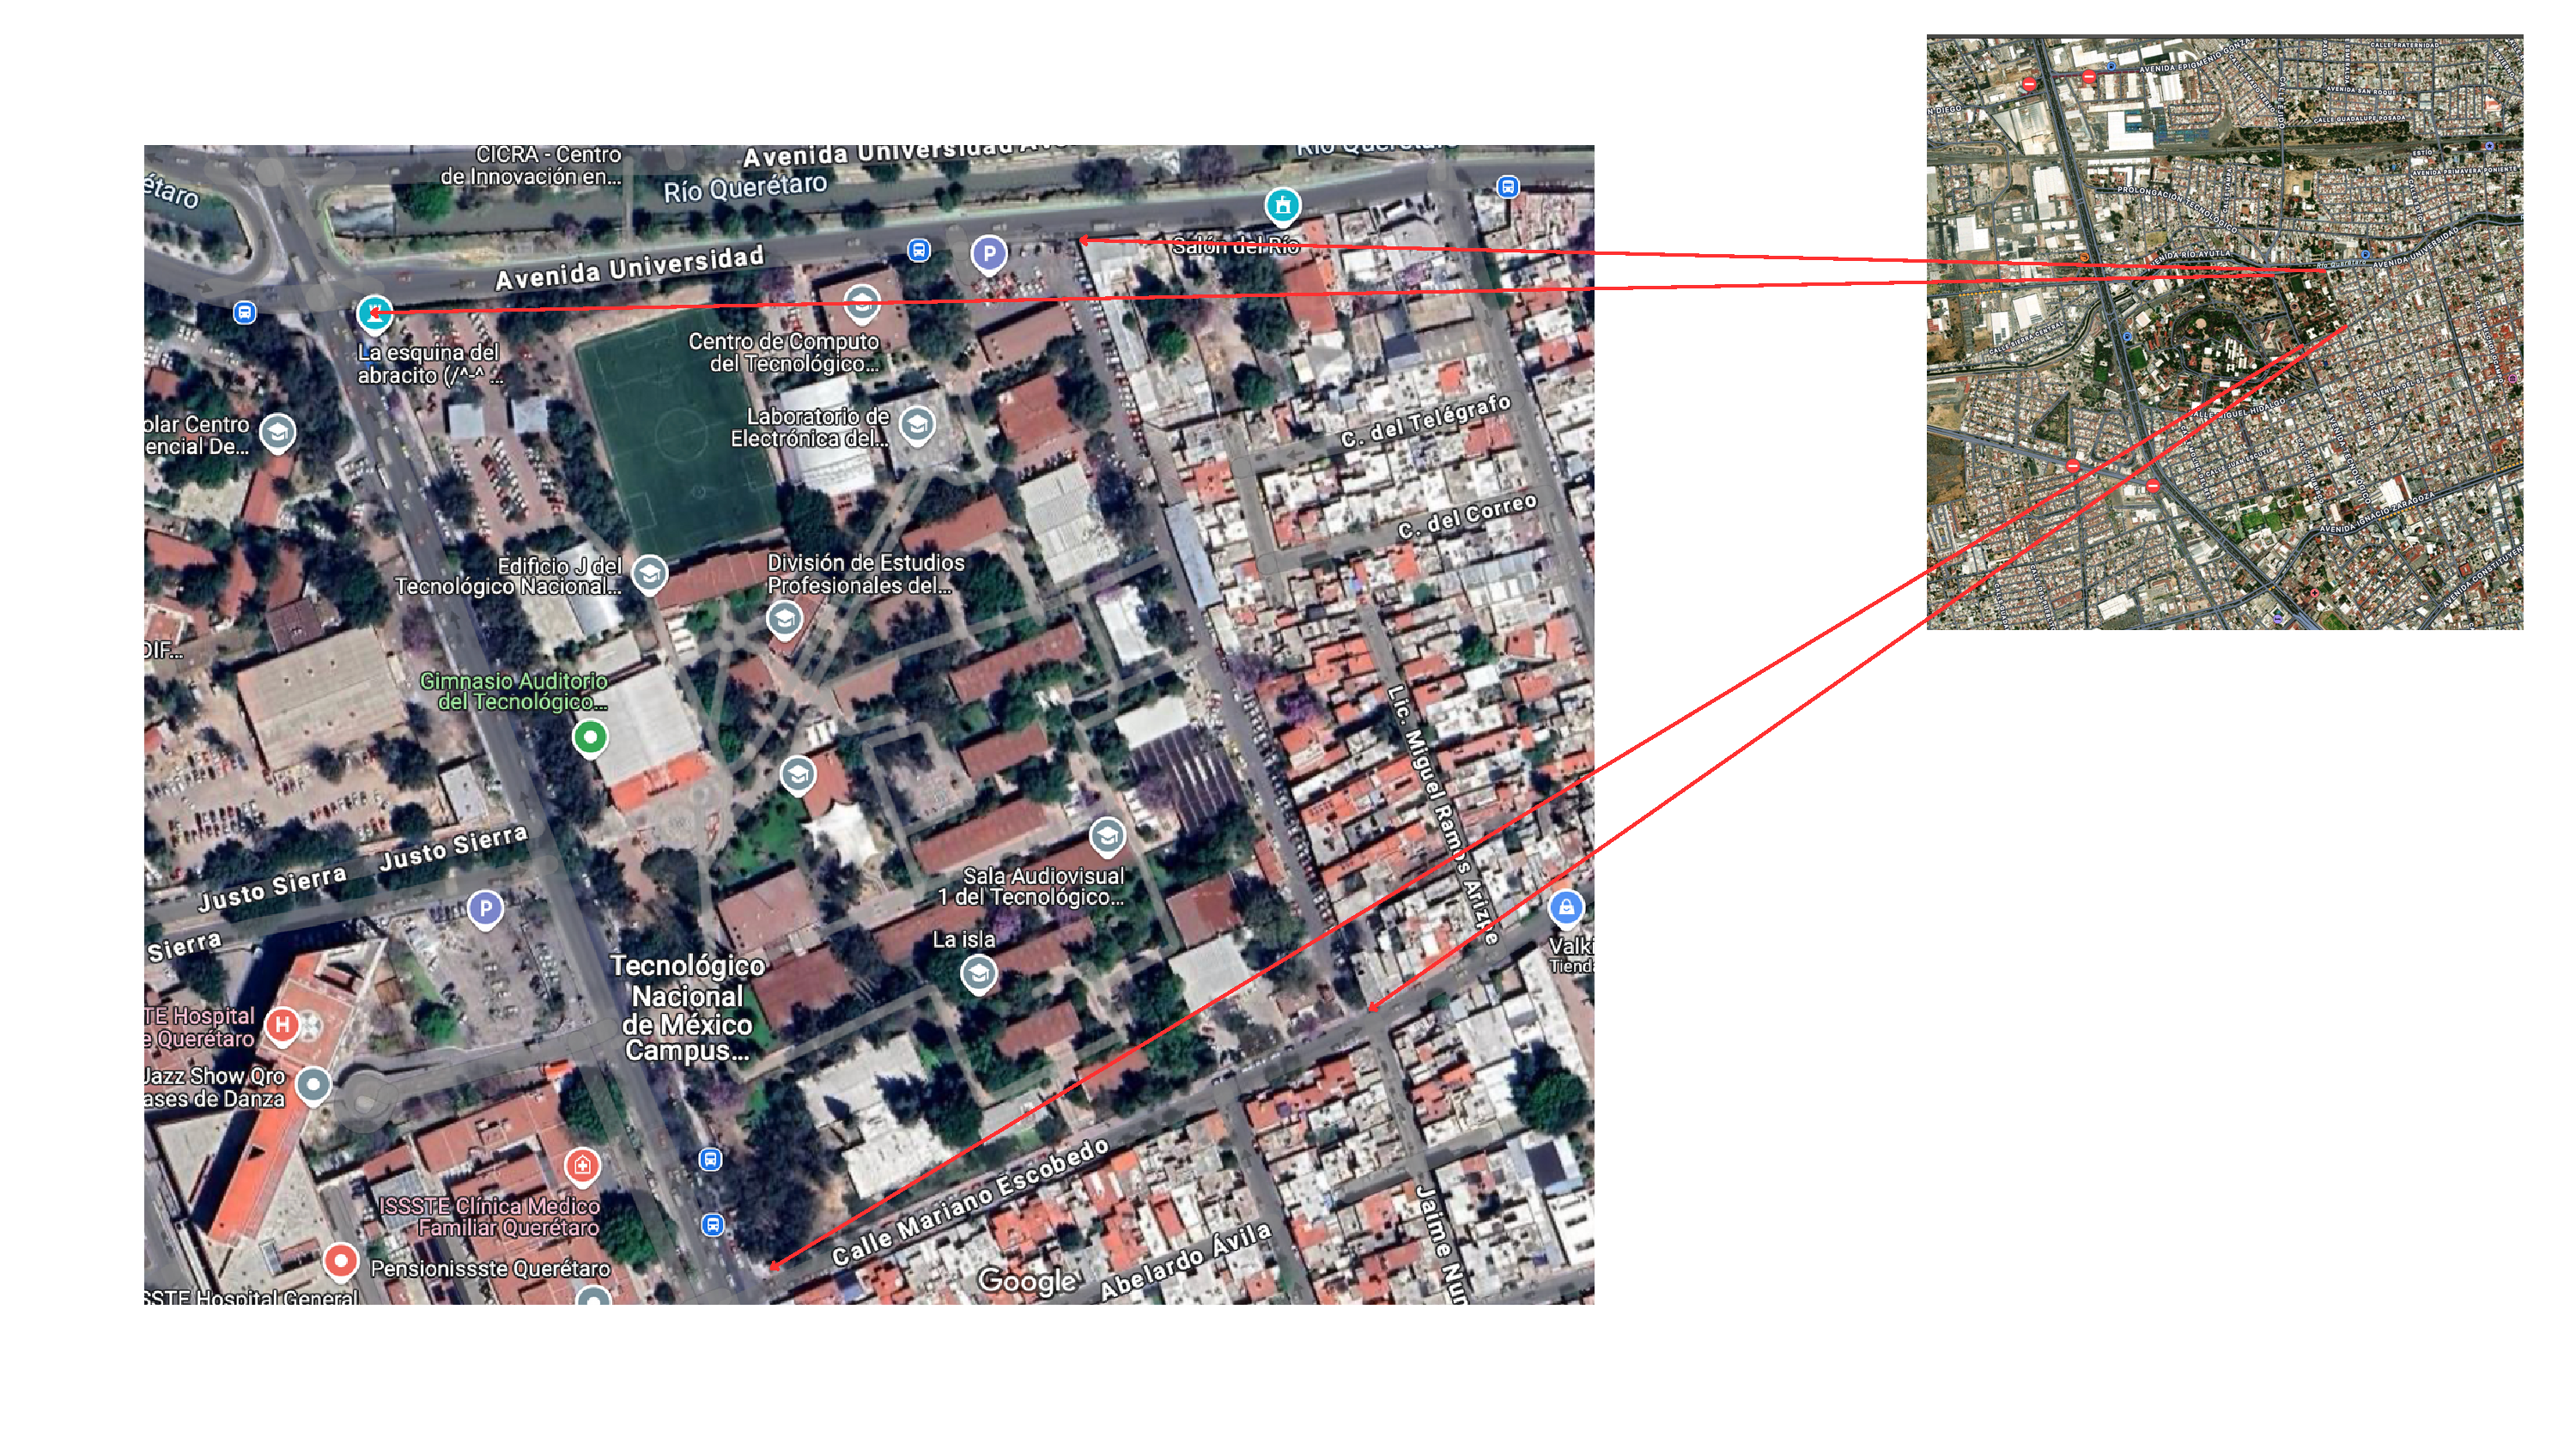
\includegraphics[scale=0.15]{15/img/mapaUbicacion.pdf}
    \caption{Instituto Tecnologico de Queretaro, Av. Tecnológivo s/n esq. Gral. Mariano Escobedo. Colonia Centro Histórico C.P. 76000, Querétaro, Querétaro, México. Tel. 442 227 4400, Correo: contacto@itq.edu.mx, Paguina Web: https://queretaro.tecnm.mx/. 
    Cuenta con una	superficie total de 78,271.42 m2 o 842,506.55 Pies2 aproximadamente, asi como un total de 5,696 estudiantes aproximadamente tanto de pregrado como posgrado y una planta academica para programas de Licenciaturas de 236 docentes y para Estudios de posgrado 6 docentes, dando uun total de 242 docentes, Dicho instituto tiene como director al Ing. Ramón Soto Arriola. }
    \label{fig:mapaUbicacion}
\end{figure}

\subsubsection{Identificación del riesgo}

Nos comprometemos a implementar diariamente un programa interno como externo de prevención de riesgos, además de solicitar retroalimentación tanto de clientes internos como externos sobre los riesgos presentes en nuestras actividades regulares. Invitamos activamente al equipo de trabajo a participar en este proceso.

Cada riesgo interno y externo será evaluado y clasificado en función de su nivel de importancia, lo que nos permitirá priorizar nuestras acciones y tomar medidas adecuadas para abordarlos véase Figura \ref{fig:nivelesDeRiesgos}.
 
\begin{figure}[H]
    \centering
    \includegraphics[scale=0.181]{15/img/diagramaIdentifiacionRiesgosAcciones.pdf}
    \caption{Diagrama para la identificación de riesgos y acciones.}
    \label{fig:diagramaIdentificacionRiesgosAcciones}
\end{figure}

\subsubsection{Riesgos internos}

El concepto de riesgo implica la probabilidad de que un evento ocurra o no, representando la cercanía de un posible daño. En términos más simples, se refiere a la probabilidad de que algo ocurra. 

Por otro lado, el riesgo operativo interno se define como la probabilidad de que la empresa experimente pérdidas debido a fallas o deficiencias en sus propios procesos o funciones naturales de operación. Específicamente, se refiere a los riesgos que surgen internamente dentro de la empresa como resultado de su propio funcionamiento.

\begin{figure}[H]
    \centering
    \includegraphics[scale=0.181]{15/img/nivelesDeRiesgos.pdf}
    \caption{Matriz de riesgos.}
    \label{fig:nivelesDeRiesgos}
\end{figure}

\begin{figure}[H]
    \centering
    \includegraphics[scale=0.181]{15/img/talaRiesgosInternos.pdf}
    \caption{Descripción de los riesgos al realizar las actividades más comunes y de riesgo dentro del aula.}
    \label{fig:tablaRiesgosInternos}
\end{figure}

% 
\subsubsection{Riesgos externos}
% 
Por otro lado, el riesgo operativo externo se define como la probabilidad de que la empresa experimente interrupciones o pérdidas debido a factores fuera de su control que afectan su funcionamiento. Específicamente, se refiere a los riesgos que surgen del entorno externo de la empresa, tales como cambios en las políticas gubernamentales, desastres naturales y situaciones de inseguridad en el área circundante. Estos riesgos provienen de influencias externas y no de deficiencias internas en los procesos o funciones de la empresa.

\begin{figure}[H]
    \centering
    \includegraphics[scale=0.17]{15/img/talaRiesgosExternos.pdf}
    \caption{Descripción de los riesgos externos.}
    \label{fig:tablaRiesgosExternos}
\end{figure}

% 
\subsubsection{Programa de actividades de prevención y auxilio}
% 
Identificamos las diversas medidas que se implementarán en respuesta a la ocurrencia de un riesgo interno o externo. Además, describimos las actividades de preparación y las disposiciones que se llevan a cabo de manera anticipada en el Instituto Tecnológico de Querétaro (ITQ) para prevenir riesgos.
% 
\subsubsection{Plan de acción}
%
Conjunto unitario de instrucciones estratégicas que habilita al ITQ para realizar una amplia gama de funciones, desde abordar problemas internos hasta gestionar riesgos externos de manera efectiva. Este plan detalla las medidas específicas que se deben tomar en caso de que surjan riesgos, tanto dentro como fuera de la institución. Incluye protocolos de respuesta claros, asignación de responsabilidades, recursos necesarios y un cronograma para su implementación. Además, el plan de acción se desarrolla de manera proactiva, mediante la identificación anticipada de posibles riesgos y la adopción de medidas preventivas para mitigar su impacto. Este enfoque proactivo garantiza que el ITQ esté preparado para hacer frente a cualquier desafío que pueda surgir, protegiendo así los intereses y la seguridad de la comunidad universitaria.

\begin{figure}[H]
    \centering
    \includegraphics[scale=0.3]{15/img/tablaPlanDeAccionRiesgosInternos.pdf}
    \caption{Descripción de las acciones anticipadas y correctivas ante un riesgo interno.}
    \label{fig:tablaPlanDeAccionRiesgosInternos}
\end{figure}

\begin{figure}[H]
    \centering
    \includegraphics[scale=0.3]{15/img/tablaPlanDeAccionRiesgosExternos.pdf}
    \caption{Descripción de las acciones anticipadas y correctivas ante un riesgo externos.}
    \label{fig:tablaPlanDeAccionRiesgosExternos}
\end{figure}

\subsubsection{Identifiación de capacidades.}
% 
%
\subsubsection{Plano de localización de recursos.}
% 
%
\subsubsection{Identifiación de apoyos externos.}
% 
\begin{figure}[H]
    \centering
    \includegraphics[scale=0.4]{15/img/tablaApoyosExternos.pdf}
    \caption{Lugares que servirán de apoyo en un situación de emergencia.}
    \label{fig:tablaApoyosExternos}
\end{figure}
%
\subsubsection{Identifiación de puntos de reunión.}
% 
\begin{figure}[H]
    \centering
    \includegraphics[scale=0.15]{15/img/mapaPuntosDeReunion.pdf}
    \caption{Zona segura en caso de una evacuación de emergencia.}
    \label{fig:mapaPuntosDeReunion}
\end{figure}
%
\subsubsection{Brigada de evacuación.}
% 
\begin{figure}[H]
    \centering
    \includegraphics[scale=0.4]{15/img/tablaBrigadaEvacuacion.pdf}
    \caption{Acciones asignadas a cada integrante del equipo de trabajo en caso de una evacuación de emergencia o repliegue.}
    \label{fig:brigada}
\end{figure}
%
\subsubsection{Directorio telefónico de emergencia.}
% 
Directorio telefónico de entidades de respuesta a emergencias y otras organizaciones implicadas en la supervisión y gestión de estas situaciones.

\begin{figure}[H]
    \centering
    \includegraphics[scale=0.35]{15/img/tablaDirectorioEmergencias.pdf}
    \caption{Números de emergencia.}
    \label{fig:tablaDirectorioEmergencias}
\end{figure}
%

\subsection{Análisis de los métodos, materiales, herramientas e instalación utilizada en la ejecución del ensamble de un circuito electrónico}
% 
\subsubsection{Planeación}

Asegúrate de conocer siempre tu objetivo.
Asegúrate de contar con los documentos (formatos, procedimientos, etc).
% 
% 
\subsubsection{5's}
% 
Consiste en tener un lugar de trabajo
más ordenado, limpio y organizado que
permite elevar la productividad y
eficiencia en una empresa, haciéndolo de manera permanente.
Las etapas son las siguientes: Seleccionar, Ordenar, Limpiar, Estandarizar, y Sostener.
% 
\subsubsection{Desarrollo del sistema de tiempos predeterminado}
%
El Sistema de Tiempos Predeterminados (STP) constituye una metodología fundamental en la ingeniería industrial, ya que facilita la optimización de procesos mediante el análisis detallado y la estandarización de los tiempos necesarios para la ejecución de tareas específicas. Este sistema se basa en los 17 Therbligs (véase en la siguiente tabla \ref{fig:tablaTherbligs}) \cite{euroinnova2024}. Los Therbligs representan los movimientos básicos en los que se puede descomponer cualquier tarea realizada en el entorno laboral. Este análisis detallado permite estudiar la productividad motriz de un operario en su estación de trabajo, proporcionando una herramienta crucial para la mejora continua y la eficiencia operativa \cite{euroinnova_therbligs}.

\begin{figure}[H]
    \centering
    \includegraphics[scale=0.25]{15/img/tablaTherblig.pdf}
    \caption{17 Therbligs.}
    \label{fig:tablaTherbligs}
\end{figure}

A partir de estos Therbligs se desarrollaron diversos sistemas que pueden ser más o menos precisos, más fáciles de aplicar, más consistentes o más adecuados para una industria específica. Teniendo origen el sistema de Métodos de Medición de Tiempos(MTM), creado por Maynard, Stegemerten y asociados. Actualmente cuenta con multiples subsistemas como los simplificados MTM-2 y MTM3 y el sistema basico MTM-1 siendo este el sistema que emplearemos a lo largo del proyecto. 

El MTM-1 es un sistema el cual analiza la operación y la desglosa en los movimientos básicos necesarios para su realización utilizando símbolos y siglas predeterminados para su identificación, además de asignar a cada movimiento básico un tiempo estándar predeterminado, basándose en su naturaleza y las condiciones en las que se lleva a cabo (TMU) véase en la Figura \ref{fig:tablaTMU}.

\begin{figure}[H]
    \centering
    \includegraphics[scale=0.6]{15/img/tablaTMU.pdf}
    \caption{Unidades de Medida De Tiempo (TMU).}
    \label{fig:tablaTMU}
\end{figure}

Movimientos MTM-1:
\begin{enumerate}
    \item Alcanzar: Se entiende como el movimiento realizado con la mano vacía, véase en la Figura \ref{fig:tabla1Alcanzar}.
    \item Mover: Transportar un objeto a un sitio, véase en la Figura \ref{fig:tabla2Mover}. 
    \item Girar y Aplicar presión: Girar la mano respecto al eje largo del antebrazo, ensamblar, véase el Caso A en la Figura \ref{fig:tabla3GirarAplicarPresion-A} y Caso B en la Figura \ref{fig:tabla3GirarAplicarPresion-B}. 
    \item Asir: Control de uno o más objetos con los dedos o manos, véase en la Figura \ref{fig:tabla4Asir}. 
    \item Colocar en Posición: Alinear, orientar o engranar un objeto con otro, véase en la Figura \ref{fig:tabla5ColocarPosicion}. 
    \item Soltar: Entregar el control de un objeto, véase en la Figura \ref{fig:tabla6Soltar}. 
    \item Desenganchar: Romper el contacto con el objeto, separar, desensamblar, véase en la Figura \ref{fig:tabla7Desenganche}. 
    \item Tiempo de Desplazamiento de ojo y Enfoque ocular: Los ojos dirigen movimientos de las manos o el cuerpo, véase en la Figura \ref{fig:tabla8TiemposDezplazamientoOjo}. 
    \item Movimientos del cuerpo (Pierna-Pie, horizontal y vertical): Los movimientos se realizan con todo el cuerpo, véase en la Figura \ref{fig:tabla9MovimietoCuerpoPie}. 
    \item Movimientos Simultáneos: Dificultad con la que se realizan los movimientos antes mencionados, véase en la Figura \ref{fig:tabla10MovimietnosSimultaneo}. 
\end{enumerate}

\begin{figure}[H]
    \centering
    \includegraphics[scale=0.32]{15/img/tabla1Alcanzar.pdf}
    \caption{Valores estandar del Therblig Alcanzar.}
    \label{fig:tabla1Alcanzar}
\end{figure}

\begin{figure}[H]
    \centering
    \includegraphics[scale=0.35]{15/img/tabla2Mover.pdf}
    \caption{Valores estandar del Therblig Mover.}
    \label{fig:tabla2Mover}
\end{figure}

\begin{figure}[H]
    \centering
    \includegraphics[scale=0.4]{15/img/tabla3GirarAplicarPresion-A.pdf}
    \caption{Valores estandar del Therblig Girar y Aplicar Presión-A.}
    \label{fig:tabla3GirarAplicarPresion-A}
\end{figure}

\begin{figure}[H]
    \centering
    \includegraphics[scale=0.6]{15/img/tabla3GirarAplicarPresion-B.pdf}
    \caption{Valores estandar del Therblig Girar y Aplicar Presión-B.}
    \label{fig:tabla3GirarAplicarPresion-B}
\end{figure}

\begin{figure}[H]
    \centering
    \includegraphics[scale=0.4]{15/img/tabla4Asir.pdf}
    \caption{Valores estandar del Therblig Asir.}
    \label{fig:tabla4Asir}
\end{figure}

\begin{figure}[H]
    \centering
    \includegraphics[scale=0.45]{15/img/tabla5ColocarPosicion.pdf}
    \caption{Valores estandar del Therblig Colocar en Posición.}
    \label{fig:tabla5ColocarPosicion}
\end{figure}
    
\begin{figure}[H]    
    \centering
    \includegraphics[scale=0.6]{15/img/tabla6Soltar.pdf}
    \caption{Valores estandar del Therblig Soltar.}
    \label{fig:tabla6Soltar}
\end{figure}

\begin{figure}[H]
    \centering
    \includegraphics[scale=0.5]{15/img/tabla7Desenganche.pdf}
    \caption{Valores estandar del Therblig Desenganchar.}
    \label{fig:tabla7Desenganche}
\end{figure}

\begin{figure}[H]
    \centering
    \includegraphics[scale=0.35]{15/img/tabla8TiempoDesplazamientoOjo.pdf}
    \caption{Valores estandar del Therblig Desplazamiento de Ojos y Enfoque Ocular.}
    \label{fig:tabla8TiemposDezplazamientoOjo}
\end{figure}

\begin{figure}[H]
    \centering
    \includegraphics[scale=0.35]{15/img/tabla9MovimientoCuerpoPie.pdf}
    \caption{Valores estandar del Therblig Movimientos del Cuerpo (Pierna-Pie, horizontal y vertical).}
    \label{fig:tabla9MovimietoCuerpoPie}
\end{figure}

\begin{figure}[H]
    \centering
    \includegraphics[scale=0.35]{15/img/tabla10MovimientoSimultaneo.pdf}
    \caption{Tablas MTM de todos los Movimientos Simultaneos.}
    \label{fig:tabla10MovimietnosSimultaneo}
\end{figure}

En base al MTM-1 y con los datos obtenidos de acuerdo a los movimientos en los que se dividieron el proceso de ensamblaje y el tiempos estandar de cada uno de ellos, obtuvimos resultados los cuales se registraron en la siguiente Hoja de análisis de métodos véase la Figura \ref{fig:tablaMTM1-1} y la Figura \ref{fig:tablaMTM1-2}.

\begin{figure}[H]
    \centering
    \includegraphics[scale=0.2]{15/img/tablaMTM1-1.pdf}
    \centering
    \includegraphics[scale=0.2]{15/img/tablaMTM1-2.pdf}
    \caption{Hoja de análisis de métodos obtenida en de acuerdo a las tablas MTM y nuestros valores.}
    \label{fig:tablaMTM1-1}
    \end{figure}
\begin{figure}[H]
    \centering
    \includegraphics[scale=0.25]{15/img/tablaMTM1-3.pdf}
    \caption{ Parte 2 de Hoja de análisis de métodos obtenida en de acuerdo a las tablas MTM y nuestros valores.}
    \label{fig:tablaMTM1-2}
\end{figure}

La ley por la que se rige el uso de los movimientos en el MTM es: ¨Principio de la reducción de movimientos¨ \cite{estudio_del_trabajo_ii}.
% 
\subsubsection{Desarrollo del muestreo del trabajo}
% 
El muestreo del trabajo es una técnica utilizada en la ingeniería industrial y en la gestión de operaciones para analizar la utilización del tiempo de trabajo y determinar la eficiencia de los procesos. Esta técnica implica observar y registrar, en momentos aleatorios, lo que están haciendo los trabajadores o cómo se están utilizando las máquinas y otros recursos. A partir de estas observaciones, se puede estimar la proporción del tiempo dedicado a diferentes actividades, tanto productivas como no productivas. En el contexto del proyecto integrador, el muestreo del trabajo se convierte en una herramienta esencial para identificar ineficiencias, cuellos de botella y oportunidades de mejora \cite{muestreo-trabajo}.
% 
\subsubsection{Corrección por balanceo de procesos}
%
La corrección por balanceo de procesos es una técnica utilizada en la gestión de operaciones y la ingeniería industrial para optimizar la distribución de trabajo a lo largo de una línea de producción o ensamble. El objetivo principal del balanceo de procesos es minimizar los tiempos de inactividad y desequilibrios entre estaciones de trabajo, asegurando que cada estación tenga una carga de trabajo equilibrada y que el flujo de producción sea lo más continuo y eficiente posible. En el proyecto integrador, aplicar el balanceo de procesos es crucial para mejorar la eficiencia y la productividad  \cite{balanceo-procesos}.
% 
\subsubsection{Datos estándar continuos y discretos}
% 
Los datos estándar continuos y discretos son dos formas de medir y representar el tiempo utilizado en procesos de producción, como el ensamblaje electrónico. Cada tipo de datos estándar tiene características específicas y se utiliza en diferentes contextos \cite{datos-estandar}.

\begin{enumerate}
    \item Datos Estándar Continuos: Estos datos representan el tiempo en unidades continuas, como minutos o segundos. Se utilizan para medir tareas que fluyen de manera continua y no se pueden dividir fácilmente en partes discretas. Por ejemplo, el tiempo necesario para ensamblar un componente electrónico puede medirse en minutos o segundos.

    \item Datos Estándar Discretos: Estos datos representan el tiempo en unidades discretas, como unidades de trabajo o movimientos individuales. Se utilizan para medir tareas que pueden descomponerse en pasos o movimientos separados. Por ejemplo, el tiempo necesario para conectar un cable en un ensamble electrónico puede medirse en unidades discretas.
 
\end{enumerate}
% 
\subsection{Diseño de la forma más económica de realizar el trabajo}
% 
El diseño de la forma más económica de realizar el trabajo es un enfoque centrado en encontrar la manera más eficiente y rentable de llevar a cabo las tareas necesarias para completar un proyecto o proceso. Esto implica identificar y utilizar métodos, materiales y recursos que minimicen los costos sin comprometer la calidad del resultado final. Dicho diseño es esencial para maximizar la eficiencia y reducir los costos asociados al ensamble de circuitos electrónicos. Esto implica examinar detenidamente cada etapa del proceso de ensamblaje para identificar oportunidades de optimización en términos de costos de materiales y recursos utilizados \cite{diseno-economico}.
% 
\subsection{Normalización de los métodos, materiales, herramientas e instalaciones}
% 
La normalización de los métodos, materiales, herramientas e instalaciones es crucial para el desarrollo de este proyecto. Este proceso implica la implementación de estándares y procedimientos uniformes que garantizan la calidad, seguridad y eficiencia en cada etapa del ensamblaje. La normalización asegura que los componentes electrónicos sean compatibles y funcionen correctamente, facilita la interoperabilidad entre diferentes partes del circuito y reduce costos al minimizar errores y retrabajos. Además, establece un marco claro para la selección de materiales, el uso de herramientas específicas y la configuración de instalaciones, lo que contribuye a la consistencia y la confiabilidad del proyecto. Al adherirse a normas establecidas, se promueve la innovación y se facilita la integración de nuevas tecnologías en el diseño y fabricación de circuitos electrónicos \cite{normalización}.

Para este proyecto se utilizaron diversos materiales, los cuales son indespensables para la obtención de un resultado positivo y los objetivos a cumplir, a continuación se muestra una lista de los materiales utilizados en tal proceso vease en la siguiente tabla \ref{fig:listaDeMateriales}.

\begin{figure}[H]
    \centering
    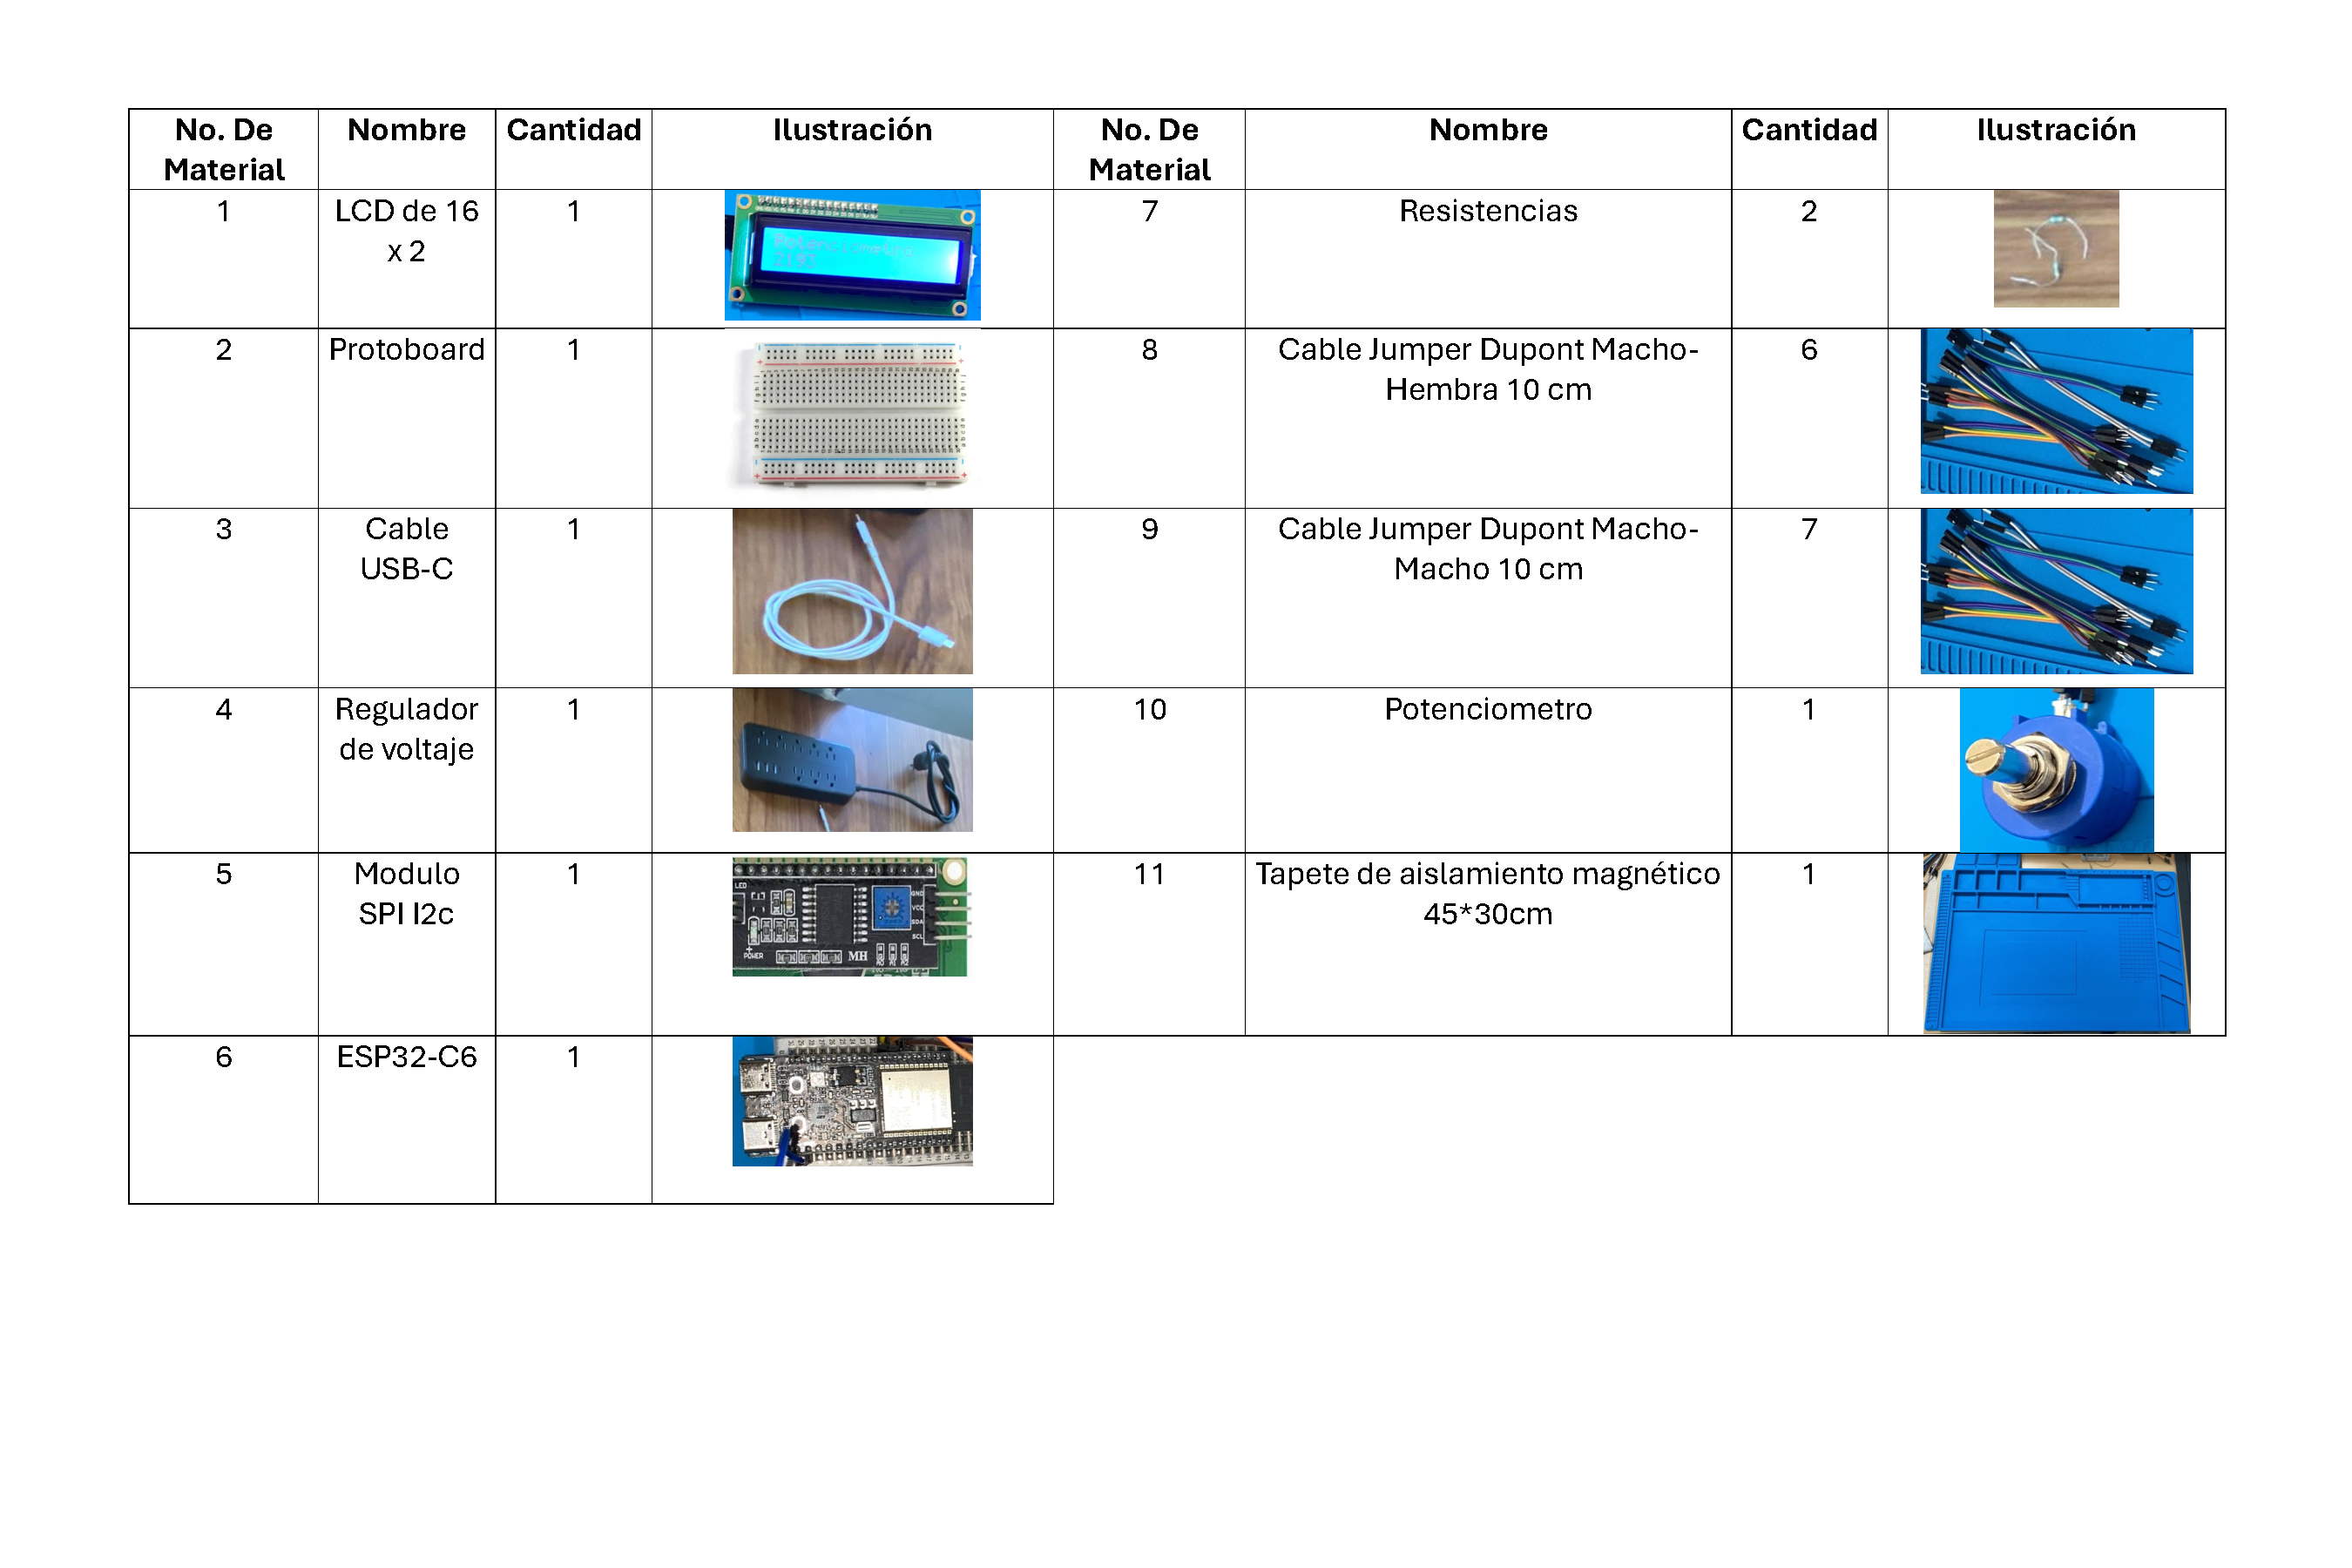
\includegraphics[scale=0.22]{15/img/listaDeMateriales.pdf}
    \caption{Lista de Materiales.}
    \label{fig:listaDeMateriales}
\end{figure}

%
\subsection{Determinación del tiempo estándar para que una persona competente realice el trabajo con marcha normal}

% 
% 
% Cada estrategia metodológica se establece acorde a cada objetivo, y por tanto deberá ser desglosada precisada y ordenada claramente. En consecuencia cada objetivo que se presentó en forma de verbo en infinitivo deberá determinar una estrategia en forma de adverbio. Ej. Desarrollar…Desarrollo. Son las actividades ordenadas que tienen como finalidad la prueba de la hipótesis. 

% \begin{itemize}
%     \item Se debe establecer que se habrá de hacer, como, conque, y donde para obtener la información que permita probar la hipótesis.  
%     \item Se debe desglosar de acuerdo a los objetivos específicos. 
%     \item Se debe establecer una estrategia metodológica por cada objetivo específico. De manera simplista se podría decir que se cambia el verbo en infinitivo por su respectivo adverbio.
%     \item En cada objetivo se debe describir que método, que materiales y que equipo se usará para conseguirlo.
%     \item Se deben tener referencias Figura \ref{fig:lcd-16x2}.
% \end{itemize}
% 
% 
% \begin{figure}[H]
%     \centering
%     \includegraphics[trim = {30mm 65mm 90mm 250mm},clip,scale=0.5]{6/Img/lcd-16x2.pdf}
%     \caption{Esquema LCD de 16x2}
%     \label{fig:lcd-16x2}
% \end{figure}
% 
% 
% \begin{figure}[H]
%     \centering
%     \includegraphics[trim = {30mm 250mm 90mm 20mm},clip,scale=0.5]{6/Img/lcd-16x2.pdf}
%     \caption{Esquema LCD de 16x2}
%     \label{fig:lcd}
% \end{figure}
% 
% 
% \subsection{Prepara tu documento}

% Antes de que comiences a utilizar esta plantilla, es recomendable que prepare la información que contendrá en un archivo aparte. 
% Ten preparadas tus gráficas, así como también las tablas aparte, para que sea más fácil integrarlo. 
% Se recomienda fuertemente el uso de \textbf{formato Enhanced Metafile (.emf) para imágenes y gráficas} de resolución óptima. 
% Finalmente, completa y organiza el contenido antes de darle el formato de esta plantilla. 

\subsection{Acrónimos y Abreviaciones}

Los acrónimos y abreviaciones deberán ser definidos únicamente la primera vez que aparecen en el texto, esto para que el lector entienda lo que significan.

% \subsection{Ecuaciones}

% Las ecuaciones son una excepción a las especificaciones prescritas de esta plantilla. 
% Deberá determinar si su ecuación debe escribirse o no utilizando la fuente Adobe Devangari. 
% Para crear ecuaciones multinivel, puede ser necesario tratar la ecuación como un gráfico e insertarla en el texto después de aplicar el estilo de la platilla.
% Las ecuaciones serán enumeradas de manera consecutiva, y el número de ecuación, entre paréntesis, se colocan al ras de la derecha, utilizando una tabulación derecha.
% 
% \begin{equation}
%     \label{eq1}
%     x + y = z 
% \end{equation}
% 
% Es importante asegurarse de que los símbolos de la ecuación sean definidos antes o inmediatamente después de la ecuación. Utilice “(1)”, en vez de “Eq. 1” al enumerar las ecuaciones, excepto al principio de una oración: “La ecuación (\ref{eq1}) es…”

\section{Resultados y discusión}

Antes de comenzar a preparar tu artículo, es importante que lea primero la guía del autor, la cual incluye los temas o apartados que son necesarios para tener tu trabajo completo.
Una vez completada la edición del texto, el documento está listo para el uso de esta plantilla. En este archivo recién creado, resalte todo el contenido e importe el archivo de texto preparado. Ahora esta listo para estilizar su documento.
En esta sección se deben presentar todo lo obtenido de la sección 2, incluidas deducciones o efectos del desarrollo. También se podrán incluir subsecciones numeradas de la siguiente forma:

\subsection{Autores y Afiliaciones}

Para distinguir las afiliaciones de los autores, utilice superíndices iniciando con el número 1, 2, etc., sucesivamente, esto dependerá de la cantidad de los departamentos a los que estén afiliados los autores. En caso de que todos los autores pertenezcan a una mismo departamento e institución, utilizar sólo el superíndice 1. 

\subsection{Identificar los encabezados}

Se les recuerda a los autores que los encabezados deben de estar conforme los solicita la guía del autor. De ahí se puede adaptar el trabajo para que sea más fácil de entender para el lector.
Los encabezados organizan los temas sobre una base relacional y jerárquica. Por ejemplo, el título del documento es encabezado del texto principal porque todo el material posterior se relaciona y elabora sobre este tema. 

\subsection{Tablas y Figuras}

\begin{enumerate}
    \item Posición de las tablas y figuras: Coloque las figuras y las tablas en la parte superior e inferior de las columnas. Evite colocarlos en medio. Las figuras y las tablas grandes pueden abarcar ambas columnas. Los títulos de las figuras deben de estar debajo de las mismas; los títulos de las tablas deben aparecer encima de ellas. Insértese las figuras y los cuadros después de citarse en el texto. Utilice la abreviatura “Fig. 1”, incluso al principio de una oración. 
\end{enumerate}

\section{Conclusiones}

Se describe aquí el alcance del trabajo, logros obtenidos y perspectivas para el futuro de este. Se sugiere colocar información cuantitativa obtenida.

\section{Agradecimientos}

Es importante darles su debido reconocimiento a los laboratorios, instituciones, organizaciones, entre otros que han sido participes para la culminación de este trabajo. También es importante mencionar, fondos, proyectos, becas, entre otros que se le han otorgado al o los autores para realizar el trabajo de investigación. Ejemplo: “Los autores agradecen al Concejo Nacional de Ciencia y Tecnología por los recursos otorgados…”
   
% \section*{Referencias}

% Para esta platilla, se solicita al autor enumerar las citas de manera consecutiva entre corchetes \cite{YLi2013}. 
% La puntuación de la oración que sigues sería \cite{Mesaelides2011}. 
% Refiérase simplemente al número de referencia, como en \cite{Morales2012}, no utilice “Ref. [3]” o “referencia [3]” excepto al principio de una oración: “La referencia [3] fue la primera…”
% Enumere las notas al pie por separado en superíndices. Coloque la nota de pie de en la parte inferior de la columna en la que se citó. No coloque notas al pie en la lista de referencias. Utilice letras para las notas al pie de la tabla.
% A menos de que haya tres autores o más; no utilice “et al.”. Los trabajos que no hayan sido publicados, incluso si han sido presentados para su publicación, deben ser citados como “inéditos”. Los trabajos que han sido aceptados para su publicación deben de citarse como “en prensa”. Poner en mayúscula sólo la primera palabra de un título, excepto los nombres propios y los símbolos de elemento. 
% Otros ejemplos \cite{LAAngeles2021}, \cite{LAAngelesConni}. 
% Véase el link \cite{prueba}, Véase el Apéndice \ref{anexo:pines}.

% Ejemplo
%  @Article{article,
% 	author = "Author1 LastName1 and Author2 LastName2 and Author3 LastName3",
% 	title = "Article Title",
% 	volume = "30",
% 	number = "30",
% 	pages = "10127-10134",
% 	year = "2013",
% 	doi = "10.3389/fnins.2013.12345",
% 	URL = "http://www.frontiersin.org/Journal/10.3389/fnins.2013.12345/abstract",
% 	journal = "Frontiers in Neuroscience"
% }

% @book{book,
%   author    = {Author Name}, 
%   title     = {The title of the work},
%   publisher = {The name of the publisher},
%   address   = {The city},
%   year      = 1993,
% }

% @incollection{chapter,
%   author       = {Bauthor Surname}, 
%   title        = {The title of the work},
%   editor       = {Editor Name},
%   booktitle    = {The title of the book},
%   publisher    = {The name of the publisher},
%   address      = {The city},
%   year         = 2002,
%   pages        = {201-213},
% }

% @InProceedings{conference,
%   author = {Cauthor Name and Dauthor Surname and Fauthor LastName},
%   title = {The title of the work},
%   booktitle = {The title of the conference proceedings},
%   year = 1996,
%   publisher = {The name of the publisher},
%   editor = {Editor Name1 and Editor Name2},
%   pages = {41-50},
% }

% @book{cho,
%   author       = {Gauthor Name1}, 
%   title        = {The title of the work},
%   publisher = {Country code and patent number},
%   address      = {Patent Country},
%   year = 2013
% }

% @book{patent,
%   author    = {Hauthor Surname1}, 
%   title     = {The title of the work},
%   publisher = {Patent number},
%   address   = {Patent country},
%   year      = 2010,
% }

% % please use misc for datasets
% @misc{dataset, 
% 	author = "Author1 LastName1 and Author2 LastName2 and Author3 LastName3",
% 	title = "Data Title",
% 	year = "2011",
% 	doi = "10.000/55555",
% 	URL = "http://www.frontiersin.org/",
% }
\bibliographystyle{ieetr}
\bibliography{15/referencias}

% 
% 
%%%%%%%%%%%%%%%%%%%%%%%%%%%%%%%%%%
\appendix
%%%%%%%%%%%%%%%%%%%%%%%%%%%%%%%%%%
% 
